\subsection{Curvature Loss}

We will define the following: \begin{center}\begin{tabular}{r|l|l}
	\(B_r\pof{e}\) & The ball of radius \(r\) around \(e\) & \(O\pof{\abs{E_G} \cdot \abs{V_M}}\) \\ \hline
	\(\mathcal{L}_{\mathrm{curvature}}\pof{M}\) & Sum of squares of the differences between vertices actual and desired curvatures & \(O\pof{\abs{E_G} \cdot \abs{V_M}}\)
\end{tabular}\end{center} Note that, in practice, the runtimes here will be significantly lower than their upper bounds since balls around edges will not typically contain a large proportion of the mesh's vertices. For example, a square mesh (as described in the main paper) with a relatively small \(\epsilon\) will have the runtimes here be closer to \(O\pof{\abs{E_G}\sqrt{\abs{V_M}}}\).

\subsubsection{Determining the Ball Around an Edge}

Before tackling the loss functional, we must determine what it means for a point to be close to an edge. Suppose \(s\) and \(s'\) are vertices in \(V_G\), and let \(e = \cof{s, s'}\). Recall that \(p_s\) (similarly \(p_{s'}\)) is the point in \(\mathbb{R}^2\) corresponding to \(s\). Define \(\pi\pof{e}\) to be the edge connecting \(p_s\) and \(p_{s'}\). We say that \(v \in B_r\pof{e}\) when \(p_v\) is within distance \(r\) of \(\pi\pof{e}\). Figure~\ref{fig:cuvature_loss_edge_ball} shows this setup.

\begin{figure}[ht]
	\centering
	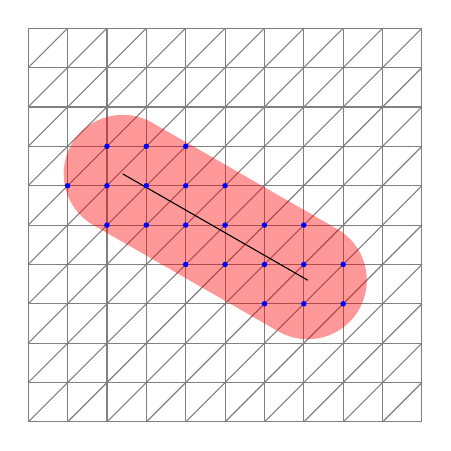
\begin{tikzpicture}[scale=0.5]
		% Draw the mesh
		\foreach \i in {0,...,9}{
			\foreach \j in {0,...,9}{
				\draw[color=gray] (\i,\j)--(\i+1,\j);
				\draw[color=gray] (\i,\j)--(\i,\j+1);
				\draw[color=gray] (\i,\j)--(\i+1,\j+1);
			}
			\draw[color=gray] (\i,10)--(\i+1,10) ;
			\draw[color=gray] (10,\i)--(10,\i+1);
		}

		% Draw the outline of the ball around the edge
		\fill[color=red, opacity=0.4] ({2.4+1.5*cos(atan((7.1-2.4)/(6.3-3.6)))},{6.3+1.5*sin(atan((7.1-2.4)/(6.3-3.6)))}) arc ({atan((7.1-2.4)/(6.3-3.6))}:{atan((7.1-2.4)/(6.3-3.6))+180}:1.5);
		\fill[color=red, opacity=0.4] ({7.1-1.5*cos(atan((7.1-2.4)/(6.3-3.6)))},{3.6-1.5*sin(atan((7.1-2.4)/(6.3-3.6)))}) arc ({atan((7.1-2.4)/(6.3-3.6))-180}:{atan((7.1-2.4)/(6.3-3.6))}:1.5);
		\fill[color=red, opacity=0.4] ({2.4-(1.5*(6.3-3.6)/sqrt((2.4-7.1)^2+(6.3-3.6)^2))},{6.3+(1.5*(2.4-7.1)/sqrt((2.4-7.1)^2+(6.3-3.6)^2))}) -- ({7.1-(1.5*(6.3-3.6)/sqrt((2.4-7.1)^2+(6.3-3.6)^2))},{3.6+(1.5*(2.4-7.1)/sqrt((2.4-7.1)^2+(6.3-3.6)^2))}) -- ({7.1+(1.5*(6.3-3.6)/sqrt((2.4-7.1)^2+(6.3-3.6)^2))},{3.6-(1.5*(2.4-7.1)/sqrt((2.4-7.1)^2+(6.3-3.6)^2))}) -- ({2.4+(1.5*(6.3-3.6)/sqrt((2.4-7.1)^2+(6.3-3.6)^2))},{6.3-(1.5*(2.4-7.1)/sqrt((2.4-7.1)^2+(6.3-3.6)^2))});

		% Draw the edge
		\draw (2.4,6.3)--(7.1,3.6);

		% Draw the points in the ball. Do this manually because automatic is too hard
		\fill[color=blue] (1,6) circle (2pt);
		\fill[color=blue] (2,5) circle (2pt);
		\fill[color=blue] (2,6) circle (2pt);
		\fill[color=blue] (2,7) circle (2pt);
		\fill[color=blue] (3,5) circle (2pt);
		\fill[color=blue] (3,6) circle (2pt);
		\fill[color=blue] (3,7) circle (2pt);
		\fill[color=blue] (4,4) circle (2pt);
		\fill[color=blue] (4,5) circle (2pt);
		\fill[color=blue] (4,6) circle (2pt);
		\fill[color=blue] (4,7) circle (2pt);
		\fill[color=blue] (5,4) circle (2pt);
		\fill[color=blue] (5,5) circle (2pt);
		\fill[color=blue] (5,6) circle (2pt);
		\fill[color=blue] (6,3) circle (2pt);
		\fill[color=blue] (6,4) circle (2pt);
		\fill[color=blue] (6,5) circle (2pt);
		\fill[color=blue] (7,3) circle (2pt);
		\fill[color=blue] (7,4) circle (2pt);
		\fill[color=blue] (7,5) circle (2pt);
		\fill[color=blue] (8,3) circle (2pt);
		\fill[color=blue] (8,4) circle (2pt);
	\end{tikzpicture}
	\caption{An overhead visualization of $B_r\pof{e}$. The mesh is in gray, $\pi\pof{e}$ is in black, and $B_r\pof{e}$ is in blue.}
	\label{fig:cuvature_loss_edge_ball}
\end{figure}

To determine whether a vertex is in the ball, we break the problem into three parts: \begin{itemize}
	\item
	Determine whether \(p_v \in B_r\pof{p_s}\). This is the case when \(\norm{p_v - p_s}_2 < r\).

	\item
	Determine whether the distance from \(p_v\) to \(\pi\pof{e}\) is less than \(r\). To do this, we first project \(p_v\) onto the line containing \(\pi\pof{e}\) to get \(p_{v, e}\): \[p_{v, e} = p_s + \frac{\pof{p_{s'} - p_s}^\intercal\pof{p_v - p_s}}{\norm{p_{s'} - p_s}_2^2}\pof{p_{s'} - p_s}.\] To determine whether this projection lies on the actual segment and that the projection is not too far away from the original point, we simultaneously check the three conditions \begin{align*}
		\pof{p_v - p_s}^\intercal\pof{p_{s'} - p_s} \ge 0, \\
		\pof{p_v - p_{s'}}^\intercal\pof{p_s - p_{s'}} \ge 0, \\
		\norm{p_v - p_{v, e}}_2 < r.
	\end{align*}

	\item
	Determine whether \(p_v \in B_r\pof{p_{s'}}\). This is the case when \(\norm{p_v - p_{s'}}_2 < r\).
\end{itemize} If any of the three above parts yields a positive response, then \(v \in B_r\pof{e}\).

% \subsection[Approximating "Fat Edges" on a Sphere]{Approximating ``Fat Edges''\footnote{This name should really be changed\dots}  on a Sphere}
% For this subsection, we will use notation that has been used elsewhere to mean other things. We do this for readability reasons.

% Consider \(u\), \(v\), and \(r\) all on the unit sphere. Assume that \(u\) and \(v\) are not antipodal. Our goal is to determine whether \(r\) is within a (geodesic) distance of \(\epsilon\) to the shortest arc between \(u\) and \(v\). If this is the case, we write \(r \in B_\epsilon\pof{\pof{u, v}}\).

% We can find the point \(\proj\pof{r}\) nearest to \(r\) on the great circle passing through \(u\) and \(v\) by projecting \(r\) onto the plane spanned by \(u\) and \(v\) and then normalizing the result. The strategy for this is to just use Graham-Schmidt to get an orthonormal basis \(\cof{v, w}\) of the plane. Once we have \(\proj\pof{r}\), we can find the distance from \(r\) to the great circle by taking advantage of the dot product.

% \begin{align*}
% 	\norm{u - \pof{u \cdot v}v}_2^2 &= \norm{u}_2^2 + \pof{u \cdot v}^2\norm{v}_2^2 - 2\pof{u \cdot v}^2 \\
% 		&= 1 + \pof{u \cdot v}^2 - 2\pof{u \cdot v}^2 \\
% 		&= 1 - \pof{u \cdot v}^2, \\
% 	w &\triangleq \frac{u - \pof{u \cdot v}v}{\norm{u - \pof{u \cdot v}v}_2}, \\
% 	\proj\pof{r} &= \frac{\pof{r \cdot v}v + \pof{r \cdot w}w}{\norm{\pof{r \cdot v}v + \pof{r \cdot w}w}_2}, \\
% 	c &\triangleq \norm{\pof{r \cdot v}v + \pof{r \cdot w}w}_2 \\
% 		&= \sqrt{\pof{r \cdot v}^2 + \pof{r \cdot w}^2} \\
% 		&= \sqrt{\pof{r \cdot v}^2 + \pof{r \cdot \frac{u - \pof{u \cdot v}v}{\norm{u - \pof{u \cdot v}v}_2}}^2} \\
% 		&= \sqrt{\pof{r \cdot v}^2 + \frac{\pof{r \cdot u - \pof{r \cdot v}\pof{u \cdot v}}^2}{1 - \pof{u \cdot v}^2}} \\
% 		&= \sqrt{\frac{\pof{r \cdot v}^2 - \pof{r \cdot v}^2\pof{u \cdot v}^2}{1 - \pof{u \cdot v}^2} + \frac{\pof{r \cdot u}^2 + \pof{r \cdot v}^2\pof{u \cdot v}^2 - 2\pof{r \cdot u}\pof{r \cdot v}\pof{u \cdot v}}{1 - \pof{u \cdot v}^2}} \\
% 		&= \sqrt{\frac{\pof{r \cdot u}^2 + \pof{r \cdot v}^2 - 2\pof{r \cdot u}\pof{r \cdot v}\pof{u \cdot v}}{1 - \pof{u \cdot v}^2}} \\
% 	 \cos\pof{\theta} &= r \cdot \proj\pof{r} \\
% 		&= \frac{\pof{r \cdot v}^2 + \pof{r \cdot w}^2}{\norm{\pof{r \cdot v}v + \pof{r \cdot w}w}_2} \\
% 		&= \norm{\pof{r \cdot v}v + \pof{r \cdot w}w}_2 \qquad \text{(by orthonormality)} \\
% 		&= c \\
% 	\theta &= \arccos\pof{c}.
% \end{align*}

% Our real question is whether \(r\) is ``close'' (within distance \(\epsilon\)) to the shortest path from \(u\) to \(v\) on the unit sphere. There are two cases to consider. The first is that \(r\) is very close to \(u\) or \(v\). This can be determined by checking \(\arccos\pof{r \cdot u} < \epsilon\) or \(\arccos\pof{r \cdot v} < \epsilon\) (if either of these is the case, then \(r\) is close).

% The second case is that \(r\) is close to some point that isn't one of the endpoints (this has some overlap with the previous case, but the previous case is easier to check, so we check it first). The trick here is to use the long computation seen above. \(r\) is close to the great circle passing through \(u\) and \(v\) when \[\arccos\pof{c} < \epsilon.\]

% Being a bit more refined, we actually want the angles between \(\proj\pof{r}\) and each of \(u\) and \(v\) to be at most the angle between \(u\) and \(v\). In other words, \begin{align*}
% 	\max\pof{\arccos\pof{\proj\pof{r} \cdot u}, \arccos\pof{\proj\pof{r} \cdot v}} &\le \arccos\pof{u \cdot v} \\
% 	\min\pof{\proj\pof{r} \cdot u, \proj\pof{r} \cdot v} &\ge u \cdot v.
% \end{align*}

% For the left hand side, we can compute
% \begin{align*}
% 	\proj\pof{r} \cdot v &= \frac{\pof{r \cdot v}v + \pof{r \cdot w}w}{\norm{\pof{r \cdot v}v + \pof{r \cdot w}w}_2} \cdot v \\
% 		&= \frac{r \cdot v}{\norm{\pof{r \cdot v}v + \pof{r \cdot w}w}_2} \\
% 		&= \frac{r \cdot v}{c}. \\
% 	\proj\pof{r} \cdot u &= \frac{r \cdot u}{c}. & \text{(by symmetry)}
% \end{align*}

% Putting this together, \(r \in B_\epsilon\pof{\pof{u, v}}\) if and only if one of the following is true:
% \begin{itemize}
% 	\item
% 	\(r \cdot u > \cos\pof{\epsilon}\);
% 	\item
% 	\(r \cdot v > \cos\pof{\epsilon}\);
% 	\item
% 	\(c > \cos\pof{\epsilon}\) and \(\min\pof{r \cdot u, r \cdot v} \ge c\,\pof{u \cdot v}\).
% \end{itemize}

\subsubsection{Forward Computation}
We have \begin{align*}
	\mathcal{L}_{\mathrm{curvature}}\pof{M} &= \frac{1}{\abs{E_G^\epsilon}}\sum_{e \in E_G^\epsilon} \sum_{\substack{k \\ v_k \in B_r\pof{e}}} \pof{\kappa_e^{\text{R}} - \kappa^{\text{G}}_k}^2.
\end{align*}

\subsubsection{Reverse Computation}
Differentiating, \begin{align*}
	\frac{\partial\pof{\mathcal{L}_{\mathrm{curvature}}\pof{M}}}{\partial\rho_\ell} &= \frac{1}{\abs{E_G}}\sum_{e \in E_G} \sum_{\substack{k \\ v_k \in B_\epsilon\pof{e}}} -2\pof{\kappa_e^{\text{R}} - \kappa^G_k}\frac{\partial\kappa^G_k}{\partial z_\ell}.
\end{align*}
